\documentclass[main.tex]{subfiles}

\begin{document}

\section*{Goal}
This week we will cover two topics. The first is how to handle vector arithmetic when we are in a more generalized case than we have covered so far. The second topic will be expanding on our investigation of forces but this week we will setup our experiment so that friction is non-negligible and therefore must be included in our calculations.

\section*{Equipment}
\begin{itemize}
\item
Force problem at lecture desk
\item
Wooden board, wood block with felt attached
\item
Mass hanger and masses
\item
Photogate Pulley
\item
String
\item
Triple-beam balance
\end{itemize}•

\section*{Theory}
\subsection*{Vector Arithmetic}
Vector arithmetic can sometimes be strange to use as it follows different rules as the regular arithmetic of real numbers we are typically used to. A vector is typically thought of as an arrow in space that has two parts: magnitude or the length of the arrow and direction or, in a flat, two-dimensional plane, the angle the arrow makes with an axis. When we add or subtract two vectors we need to take both parts into consideration.
\begin{figure}[h]
\centering
\begin{tikzpicture}[
	Vect1/.style={draw=red,fill=red,thick,>=latex},
	Vect2/.style={draw=blue,fill=blue,thick,>=latex},
	Vect3/.style={draw=brown,fill=brown,thick,>=latex}
]

\coordinate (O) at (0,0);
\coordinate (A) at (2,1);
\coordinate (B) at (5,0);
\draw[Vect1,->] (O) -- (A) node [midway, above] {$\mathbf{A}$};
\draw[Vect2,->] (A) -- (B) node [midway, above] {$\mathbf{B}$};
\draw[Vect3,->] (O) -- (B) node [midway, below] {$\mathbf{C}=\mathbf{A}+\mathbf{B}$};

\tikzAngleOfLine(A)(O){\AngleStart}
\tikzAngleOfLine(A)(B){\AngleEnd}

\draw (A)+(\AngleStart:0.25cm) arc (\AngleStart:\AngleEnd:0.25cm);
\node [below] at ($(A)+({(\AngleStart+\AngleEnd)/2}:0.25 cm)$) {$\alpha$};

\end{tikzpicture}
\caption{} \label{fig:LawCosines}
\end{figure}
For example consider the vector addition in Figure~\ref{fig:LawCosines}. In order to find the magnitude of vector $\mathbf{C}$ we would need to know the magnitudes $A=|\mathbf{A}|$ and $B=|\mathbf{B}|$ and the angle between them, $\alpha.$ We remember from trigonometry that to find the length of the third side of any triangle, we use the law of cosines,
\begin{equation}\label{eq:LawofCosines}
C=\sqrt{A^2+B^2-2AB\cos\alpha}.
\end{equation}
Using Equation~\eqref{eq:LawofCosines} we can find $C$ but it can sometimes lead to confusion as to how the angle $\alpha$ is defined in relation to the angles $\theta_A$ and $\theta_B$ that define the orientation of vectors $\mathbf{A}$ and $\mathbf{B}$ respectively. Also, while Equation~\eqref{eq:LawofCosines} is simple now, with the addition of more than two vectors our job can become much more difficult. So instead of using the law of cosines, let us develop another method that is more procedural and easier to follow.

\begin{wrapfigure}{R}{0.5\textwidth}
\vspace{-10pt}
\centering
\begin{subfigure}[h]{0.5\textwidth}
\centering
\begin{tikzpicture}[
	Vect1/.style={draw=red,fill=red,thick,>=latex},
	Vect2/.style={draw=blue,fill=blue,thick,>=latex},
	Vect3/.style={draw=brown,fill=brown,thick,>=latex},
	axis/.style={draw=black,fill=black,>=latex}
]
	
	\draw[axis,->] (-0.5,0) -- (3,0) node [right] {$x$};
	\draw[axis,->] (0,-0.5) -- (0,3.5) node [above] {$y$};
	
	\coordinate (O) at (0,0);
	\coordinate (A) at (1,1); \coordinate (Ax) at (1,0); \coordinate (Ay) at (0,1);
	\coordinate (B) at (2,3); \coordinate (Bx) at (2,0); \coordinate (By) at (0,3);
	\coordinate (Y) at (3,1);
	
	\draw[Vect3,->] (O) -- (B) node [midway, above,xshift=-3pt] {$\mathbf{C}$};
	\draw[Vect1,->] (O) -- (A) node [midway, above,xshift=-3pt] {$\mathbf{A}$};
	\draw[Vect2,->] (A) -- (B) node [midway, above,xshift=-5pt] {$\mathbf{B}$};
	
	\draw[Vect1,->] (O) -- (Ax) node [midway, below] {$A_x$};
	\draw[Vect1,->] (O) -- (Ay) node [midway, left] {$A_y$};
	\draw[Vect2,->] (Ax) -- (Bx) node [midway, below] {$B_x$};
	\draw[Vect2,->] (Ay) -- (By) node [midway, left] {$B_y$};
	
	\draw [decorate,decoration={brace,amplitude=10pt,mirror},xshift=0pt,yshift=-3pt] (0,-0.5) -- (2,-0.5) node [midway, below, yshift=-10pt] {$C_x$};
	\draw [decorate,decoration={brace,amplitude=10pt},xshift=-3pt,yshift=0pt] (-0.5,0) -- (-0.5,3) node [midway, left, xshift=-10pt] {$C_y$};
	
	\draw[dashed,gray] (A) -- (Ax);
	\draw[dashed,gray] (Ay) -- (Y);
	\draw[dashed,gray] (B) -- (By);
	\draw[dashed,gray] (B) -- (Bx);
	
	\tikzAngleOfLine(O)(A){\AngleStartA}
	\tikzAngleOfLine(O)(Ax){\AngleEndA}
	\tikzAngleOfLine(A)(B){\AngleStartB}
	\tikzAngleOfLine(A)(Y){\AngleEndB}
	
	\draw (O)+(\AngleStartA:0.25cm) arc (\AngleStartA:\AngleEndA:0.25cm);
	\node [right,yshift=3pt] at ($(O)+({(\AngleStartA+\AngleEndA)/2}:0.25 cm)$) {$\theta_A$};
	\draw (A)+(\AngleStartB:0.25cm) arc (\AngleStartB:\AngleEndB:0.25cm);
	\node [right,yshift=5pt] at ($(A)+({(\AngleStartB+\AngleEndB)/2}:0.25 cm)$) {$\theta_B$};

\end{tikzpicture}
\caption{} \label{fig:Example}
\end{subfigure}

\begin{subfigure}[h]{0.5\textwidth}
\centering
\begin{tikzpicture}[
	scale=1.5,
	Vect1/.style={draw=red,fill=red,thick,>=latex},
	axis/.style={draw=black,fill=black,>=latex}
]
	
	\draw[axis,->] (-0.5,0) -- (1.5,0) node [right] {$x$};
	\draw[axis,->] (0,-0.5) -- (0,1.5) node [above] {$y$};

	\coordinate (O) at (0,0);
	\coordinate (A) at (1,1); \coordinate (Ax) at (1,0); \coordinate (Ay) at (0,1);

	\draw[Vect1,->] (O) -- (A) node [midway, above,xshift=-3pt] {$\mathbf{A}$};

	\draw[Vect1,->] (O) -- (Ax) node [midway, below] {$A_x$};
	\draw[Vect1,->] (Ax) -- (A) node [midway, right] {$A_y$};

	\tikzAngleOfLine(O)(A){\AngleStartA}
	\tikzAngleOfLine(O)(Ax){\AngleEndA}

	\draw (O)+(\AngleStartA:0.25cm) arc (\AngleStartA:\AngleEndA:0.25cm);
	\node [right,yshift=3pt] at ($(O)+({(\AngleStartA+\AngleEndA)/2}:0.25 cm)$) {$\theta_A$};
	\draw (.85,0) -- (.85,.15) -- (1,.15);

\end{tikzpicture}
\caption{} \label{fig:VectA}
\end{subfigure}
\caption{}
\vspace{-9\baselineskip}
\end{wrapfigure}

Consider the vectors in Figure~\ref{fig:Example}, We want to compute both the magnitude of vector $\mathbf{C}$ and its angle $\theta_C.$ To do this we must first break the vectors $\mathbf{A}$ and $\mathbf{B}$ into their $x$ and $y$ components. The advantage of this is that instead of dealing with an obtuse triangle we can focus on one right triangle per vector, which is much easier to handle and can easily be expanded to as many vectors as we need.
\FloatBarrier

To determine the components of our vectors we use the basic trigonometric identities,
\begin{align}
\cos\theta_A=\frac{A_x}{A} \; \text{or} \; A_x=A\cos\theta_A,\\
\sin\theta_A=\frac{A_y}{A} \; \text{or} \; A_y=A\sin\theta_A.
\end{align}
Once we have reduced all our vectors to components along the axes, we can then simply add the components that are in the same direction to get the components of our resultant vector, $\mathbf{C}.$ When we have our resultant components, we can use the Pythagorean theorem to find the magnitude of our resultant,
\begin{align}
C&=\sqrt{C_x^2+C_y^2}\nonumber\\
&=\sqrt{(A_x+B_x)^2+(A_y+B_y)^2}.
\end{align}
To find the the direction, we use the identity,
\begin{equation}
\tan\theta_C=\frac{C_y}{C_x} \quad \text{or} \quad \theta_C=\arctan\left(\frac{C_y}{C_x}\right).
\end{equation}
n.b., While we may often use degrees to measure angles out of habit or convenience in physics it should be noted that the standard unit for an angle is a radian, where $1\text{ rad} = 57.3\degree.$
\FloatBarrier

\subsection*{Kinetic Friction}
In our kinetic friction experiment we will use the same setup as last time, but with one important difference. Whereas last time we used the dynamics track and cart to minimize friction, this time we will use a block of wood against a plank of wood to generate a noticeable frictional force.

\begin{wrapfigure}{r}{0.5\textwidth}
\centering
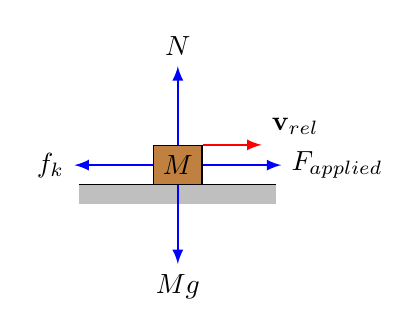
\begin{tikzpicture}[
	m/.style={rectangle,draw=black,fill=brown,minimum size=0.5cm,thin},
	force/.style={>=latex,draw=blue,fill=blue,thick},
	velocity/.style={>=latex,draw=red,fill=red,thick}
]

	\node[m] (m) {$M$};
	\fill[lightgray] (-1.25,-0.25) rectangle (1.25,-0.5);
	\draw (-1.25,-0.25) -- (1.25,-0.25);

	\draw[force,->] (m.north) -- ++(0,1) node [above] {$N$};
	\draw[force,->] (m.east) -- ++ (1,0) node [right] {$F_{applied}$};
	\draw[force,->] (m.south) -- ++(0,-1) node [below] {$Mg$};
	\draw[force,->] (m.west) -- ++(-1,0) node [left] {$f_k$};

	\draw[velocity,->] (m.north east) -- ++(0.75,0) node [above right] {$\mathbf{v}_{rel}$};

\end{tikzpicture}
\caption{} \label{fig:Friction}
\end{wrapfigure}
The frictional force $\boldsymbol{f}$ describes a force that opposes the velocity of the body relative to its frictional substrate. In common cases, the relative velocity $\mathbf{v}_{rel}$ is generated by an applied force, so $F_{applied}$ and $\mathbf{v}_{rel}$ point in the same direction, as in Figure~\ref{fig:Friction}. The frictional force can be experimentally found to be be approximately proportional to the \emph{magnitude} of of the normal force by the relation,
\begin{equation} \label{eq:Friction}
f_k=\mu_kN,
\end{equation}
where $\mu_k$ is a constant called the \emph{coefficient of kinetic friction}. In reality Equation~\eqref{eq:Friction} is only an approximation because $\mu_k$ may depend in a complicated way on system properties such as temperature and velocity.  For the purposes of our experiment however we will consider that $\mu_k$ \emph{is dependent on the materials involved} and possibly on a few other variables that we will check in today's experiment.

As in Chapter~\ref{chap:Force}, we consider a mass $M$ moving on a horizontal surface and pulled into motion by the weight of a vertically hanging mass $m.$ If we set up our force diagram as we did last time we can get the system of equations,
\begin{subequations}
\begin{align}
M: 	\sum F_x &= T-f_k=Ma\\
	\sum F_y &=N-Mg=0\\
m:	\sum F_x &=0\\
	\sum	F_y &=T-mg=-ma,
\end{align}
\end{subequations}
which we can, with some work, find an expression for the coefficient of kinetic friction as,
\begin{equation} \label{eq:muk}
\mu_k=\frac{mg-(M+m)a}{Mg}.
\end{equation}•

\section{Setup I: Vector Arithmetic}
\begin{enumerate}
\item
Use the three forces assigned by the instructor to solve for the resultant vector $\mathbf{D}=\mathbf{A}+\mathbf{B}+\mathbf{C}$ by using the component method described in the theory section. Record the values on the data sheet. Show sample calculations.
\item
Use the additional pair of forces assigned by the instructor to calculate the resultant vector $\mathbf{C}=\mathbf{A}-\mathbf{B}$ by using the component method. Hint: $\mathbf{A}-\mathbf{B}=\mathbf{A}+ (-\mathbf{B})$ where $-\mathbf{B}$ has the same magnitude as $\mathbf{B}$ but is in the opposite direction, e.g., if for $\mathbf{B}$ the components are $B_x=2\text{ N}$ and $B_y=5\text{ N}$ then $-\mathbf{B}$ has components $B_x=-2\text{ N}$ and $B_y=-5\text{ N}.$
\item \label{step:UnknownMass}
At the lecture table, a problem has been setup with an unknown mass. Measure the angles and record the tension along the strings making sure that we convert the reading of the scale (in grams) into a force (in Newtons). Using vector arithmetic, solve for the unknown mass. (Hint: The point of the string from which the weight is suspended is not moving. What does that tell us have the net vector force acting on that point?)
\end{enumerate}

\section{Setup II: Kinetic Friction}
For this setup, the Photogate Pulley will measure the motion of the block sliding on a horizontal surface. The block is connected by a string to a hanging mass, We will vary the mass, surface area of the block, the type of material between the block and the surface, and the amount of hanging mass to change the circumstances of the block. Capstone will then record and display the data by plotting the speed vs time, the slope of which will be the average acceleration of the block for each trial.
\begin{enumerate}
\item
Start Capstone.
\item
Mount the Photogate Pulley at the edge of the board and table top as shown.

\includegraphics[width=\textwidth]{Friction_Setup}

\item
Attach the Photogate Pulley to the 850UI.
\item
Under ``Hardware Setup" connect the ``Photogate with Pulley" in the appropriate port. Click ``Hardware Setup" to hide it.
\item
Double-click ``Graph" in the toolbar on the right.
\item
For the vertical axis choose ``Linear Speed (m/s)."
\end{enumerate}•

\subsection*{Procedure}
\begin{enumerate}
\item
Measure and record the mass of the block of wood ($M$).
\item
Use a piece of string that is about 10 cm longer than the distance from the top of the board to the floor. Attach one end to the string to the block. Attach the mass hanger to the other end of the string.
\item \label{step:LargeSmooth}
Run \#1 \& \#2---Large, Smooth Surface
\begin{enumerate}
\item \label{step:LargeSmooth_start}
Place the block so its largest smooth surface is on the horizontal surface.
\item
Put enough mass on the the mass hanger so that the block will slide on the surface without needing an initial push. Measure and record the value of the total hanging mass ($m$).
\item
Pull the block away from the Photogate Pulley until the hanging mass is almost up to the pulley. Hold the block in place. Turn the pulley so the Photogate's beam is not blocked. (The LED on the Photogate will be off when the beam is clear.)
\item \label{step:LargeSmooth_end}
Click on the Record button and release the block. Click on the Stop button to end data collection just before the block hits the pulley. Stop the block so that it does not hit the Photogate Pulley.
\item
Repeat steps~\ref{step:LargeSmooth_start}--\ref{step:LargeSmooth_end}.
\end{enumerate}
\item
Run \#3---Different Mass of Block
\begin{enumerate}
\item
Double the mass of the block by placing a mass approximately equal to that of the block on top of the block.
\item
Measure and record the total mass of the block system ($M$).
\item
Double the hanging mass. Measure and record the total hanging mass ($m$).
\item
Repeat steps~\ref{step:LargeSmooth_start}--\ref{step:LargeSmooth_end}.
\end{enumerate}•
\item
Run \#4---Different Surface Area
\begin{enumerate}
\item
Remove the extra mass from the block.
\item
Place the block so that its smallest smooth side is on the horizontal surface. Adjust the height of the Photogate Pulley so that the string remains level with the horizontal surface.
\item
Use the same hanging mass we used in step~\ref{step:LargeSmooth} (\emph{not} Run \#3) so we can compare the runs.
\item
Repeat steps~\ref{step:LargeSmooth_start}--\ref{step:LargeSmooth_end}.
\end{enumerate}•
\item
Runs \#5 \& \#6---Different Hanging Mass
\begin{enumerate}
\item
Return the block so the largest smooth side is on the horizontal surface.
\item
Put an amount of mass on the hanger that is larger than the amount we used in step~\ref{step:LargeSmooth}. Measure and record the total hanging mass ($m$).
\item
Repeat steps~\ref{step:LargeSmooth_start}--\ref{step:LargeSmooth_end}.
\item
Repeat the process using two larger hanging masses each larger than the previous. Measure and record the total hanging mass ($m$) each time.
\end{enumerate}•
\item
Runs \#7--\#9---Different Surface Material 
\begin{enumerate}
\item
Place the block so that its largest rough side is on the horizontal surface.
\item
Put enough mass on the mass hanger so that the block will slide on the surface without needing an initial push. Measure and record the value of the total hanging mass ($m$).
\item
Repeat steps~\ref{step:LargeSmooth_start}--\ref{step:LargeSmooth_end} to see how the different material affects the coefficient of kinetic friction.
\item
Place the block so its smallest rough side is on the horizontal surface.
\item
Repeat steps~\ref{step:LargeSmooth_start}--\ref{step:LargeSmooth_end} using the same hanging mass as we did for the largest rough side so we can compare the two runs.
\end{enumerate}•
\end{enumerate}•

\subsection*{Analysis}
\begin{enumerate}
\item \label{step:FrictionAnalysis_start}
Using the Select Data Run button \includegraphics{Select_Data_Run} display only Run \#1.
\item
For all data runs we will use a linear fit. The slope of the fit line will be the average acceleration of the block.
\item
If necessary, use the Selection Tool \includegraphics{Selection_Tool} to highlight only the relevant portion of the data. 
\item \label{step:FrictionAnalysis_end}
Record the acceleration in the data table.
\item
\textbf{Print} a copy of the graph for all group members.
\item
Repeat steps~\ref{step:FrictionAnalysis_start}--\ref{step:FrictionAnalysis_end} for each of the remaining runs.
\item
Calculate $\mu_k$ for each run using Equation~\eqref{eq:muk}.
\item
Calculate and record on the data table for Runs \#1 and \#2 the mean value of $\mu_k,$ and the discrepancy between the two values. We will take this discrepancy as indicating the typical experiment error in all our measurements of $\mu_k.$ (Of course, it may happen to be unusually small or large, but this is the best we can do with our present set of measurements.)
\item
Calculate an record all the percent discrepancies of $\mu_k$ relative to $\mu_{k0},$ namely,
\[
\left(\frac{\mu_k}{\mu_{k0}-1}\right)100\%.
\]
\end{enumerate}

\begin{question}
How does the coefficient of kinetic friction vary with the mass of the block? Is this variation significant? (By ``significant," we mean that \emph{the percent discrepancy is more than twice the percent error.} If our answer is ``No, it is not significant," then we are saying that, within the limits of measurement error, $\mu_k$ can be taken as a constant.
\end{question}
\begin{question}
How does the coefficient of kinetic friction vary with the area of contact between the block and the horizontal surface? Is this variation significant?
\end{question}
\begin{question}
How does the coefficient of kinetic friction vary with the type of material between the block and the horizontal surface? Is this variation significant?
\end{question}
\begin{question}
When we used the different type of material, how does the coefficient of kinetic friction vary with the area of contact between the block and the horizontal surface? Is this variation significant?
\end{question}
\begin{question}
How does the coefficient of kinetic friction vary as the speed varied due to the different hanging masses? Is this variation significant?
\end{question}
\begin{question}
When the mass of the block is increased, does the force of kinetic friction increase? Why?
\end{question}

\begin{samepage}
\hrulefill \\
\emph{Week Four:} \textbf{Vectors \& Kinetic Friction}
\begin{enumerate}
\item
\textbf{(1)} Title Page
\item
\textbf{(5)} Purpose of Kinetic Friction
\item
\textbf{(8)} Theory for Kinetic Friction---Should include a free-body diagram.
\item
\textbf{(2)} Data Sheet for Kinetic Friction
\item
\textbf{(4)} Sample Calculations for Kinetic Friction
\item
\textbf{(1)} Graph from Kinetic Friction
\item
\textbf{(12)} Answers to questions.
\item
\textbf{(9)} Calculations and free-body diagram for step~\ref{step:UnknownMass} in Vector Arithmetic section.
\item
\textbf{(9)} Data Sheet for Vector Arithmetic section.
\end{enumerate}•

\newpage
\begin{doublespace}
\section{Data Sheets}
\subsection*{Vector Arithmetic}

\begin{centering}
$\mathbf{A}=\rule[-1mm]{2.5cm}{.1pt}\text{ at }\rule[-1mm]{2.5cm}{.1pt}$\\
$\mathbf{B}=\rule[-1mm]{2.5cm}{.1pt}\text{ at }\rule[-1mm]{2.5cm}{.1pt}$\\
$\mathbf{C}=\rule[-1mm]{2.5cm}{.1pt}\text{ at }\rule[-1mm]{2.5cm}{.1pt}$\\
\end{centering}\vspace{10pt}

\begin{tabular}{|c|c|c|}
\hline
Vector & $x$ Component & $y$ Component\\
\hline
&&\\
\hline
&&\\
\hline
&&\\
\hline
Resultant ($\mathbf{D}=\mathbf{A}+\mathbf{B}+\mathbf{C}$) &&\\
\hline
\end{tabular}•\\

Magnitude$=\rule[-1mm]{2.5cm}{.1pt} \quad  \tan\theta=\rule[-1mm]{2.5cm}{.1pt} \quad \theta=\rule[-1mm]{1.5cm}{.1pt}$\\

\begin{centering}
$\mathbf{A}=\rule[-1mm]{2.5cm}{.1pt}\text{ at }\rule[-1mm]{2.5cm}{.1pt}$\\
$\mathbf{B}=\rule[-1mm]{2.5cm}{.1pt}\text{ at }\rule[-1mm]{2.5cm}{.1pt}$\\
\end{centering}\vspace{10pt}

\begin{tabular}{|c|c|c|}
\hline
Vector & $x$ Component & $y$ Component\\
\hline
&&\\
\hline
&&\\
\hline
Resultant ($\mathbf{C}=\mathbf{A}-\mathbf{B}$) &&\\
\hline
\end{tabular}•\\ \\

Lecture Table Problem:\\
$F_1=\rule[-1mm]{2.5cm}{.1pt}, \theta_1=\rule[-1mm]{1.5cm}{.1pt} \quad F_2=\rule[-1mm]{2.5cm}{.1pt}, \theta_2=\rule[-1mm]{1.5cm}{.1pt}$

\newpage
\subsection*{Kinetic Friction}
\begin{tabbing}
Mass of block ($M$):\= \rule[-1mm]{2.5cm}{.1pt}kg (Except Run \#3)\\
\>\rule[-1mm]{2.5cm}{.1pt}kg (Run \#3)
\end{tabbing}

Run \#1 and \#2 only:\\
\begin{tabular}{ll}
Average value of $\mu_k$:& $\mu_{k0}:\rule[-1mm]{2.5cm}{.1pt}$\\
Percent discrepancy of $\mu_k$:& \%-Error:\rule[-1mm]{2.5cm}{.1pt}
\end{tabular}\\


\begin{tabular}{|c|c|c|c|c|}
\hline
Run \# & Hanging Mass $m$ (kg) & Acceleration $a\; (\text{m}/\text{s}^2)$ & Coefficient $\mu_k$ & \%-Discrep of $\mu_k$\\
\hline
1 &&&&\Vhrulefill\\
\hline
2 &&&&\Vhrulefill\\
\hline
3 &&&&\\
\hline
4 &&&&\\
\hline
5 &&&&\\
\hline
6 &&&&\\
\hline
7 &&&&\\
\hline
8 &&&&\\
\hline
9 &&&&\\
\hline
\end{tabular}•
\end{doublespace}

\end{samepage}

\end{document}
